\documentclass{../../PublicResources/DocClass}

    \DocumentTitle{文档标题测试}
    \DocumentSubtitle{文档副标题测试}
    \DocumentCreatedDate{2020/7/21}

    \LinkBlogPost{https://test.link1/}
    \LinkPDFSource{https://test.link2/}
    \LinkVideo{https://test.link3/}

    \AuthorName{Mr. Kin}
    \AuthorEmail{im.misterkin@gmail.com}
    \AuthorBlog{https://mister-kin.github.io/}

\begin{document}
    \pagenumbering{Roman} % 大写罗马字母样式页码。
    \maketitle
    \addcontentsline{toc}{chapter}{封面}
    \frontmatter
    \phantomsection
\begin{center}
    {\bfseries\sffamily\Large 关于作者}
\end{center}
\addcontentsline{toc}{chapter}{关于作者}

\subsection*{\bfseries \sffamily 关于我}
\begin{wrapfigure}[3]{L}{60pt}
    \vspace*{-20pt}
    \centering
    
\includegraphics{kin-logo}
\end{wrapfigure}
\textbf{Mr. Kin},广东客家仁,程序猿,CG和游戏爱好者,一枚极客。翻译UP主,个人UP主。不定时在B站直播日常:码代码,码博客,翻译,做视频,做教程。 ($\vartheta$$\bullet$\_$\bullet$)$\vartheta$ \hyperlink{follow}{\emph{(点击关注我!)}}

\subsection*{\bfseries \sffamily 开源建设}

\noindent {\bfseries \sffamily 开源软件的中文化翻译}

\begin{itemize}
    \item \href{https://docs.krita.org/zh_CN/}{Krita手册}:2018.8.5 - \href{https://crowdin.com/profile}{2019.4.23}
    \item \href{https://docs.blender.org/manual/zh-hans/latest/}{Blender手册}:2019.7.20 - \href{https://www.blendercn.org/5812.html?tdsourcetag=s_pctim_aiomsg}{2019.9.4} - 至今(\href{https://developer.blender.org/p/Mr_Kin/}{翻译维护})
\end{itemize}

\subsection*{\bfseries \sffamily \hypertarget{contact}{联系方式}}
\vspace*{-1ex}
\noindent {\footnotesize \color{red} \em 注:联系时请注明身份,谢谢!}

\begin{itemize}
    \item QQ:\href{tencent://AddContact/?fromId=45&fromSubId=1&subcmd=all&uin=2312463626&website=www.oicqzone.com}{2312463626}\emph{\color{red}(点击号码加好友)}
    \item 邮箱:2312463626@qq.com ; im.misterkin@gmail.com
\end{itemize}

\subsection*{\bfseries \sffamily \hypertarget{follow}{关注渠道}}
\vspace*{-1ex}
\noindent {\footnotesize \color{red} \em 注:点击文字即可跳转关注!}
\vspace*{-2ex}

\begin{figure}[htbp]
    \centering
    
\includegraphics[scale=0.2]{WechatOfficialAccounts.png}
\end{figure}
\vspace*{-4ex}

\begin{figure}[htbp]
    \centering
    \begin{minipage}[t]{0.2\textwidth}
        \centering
        \caption*{\href{https://mister-kin.github.io}{博客 - Blog}}
        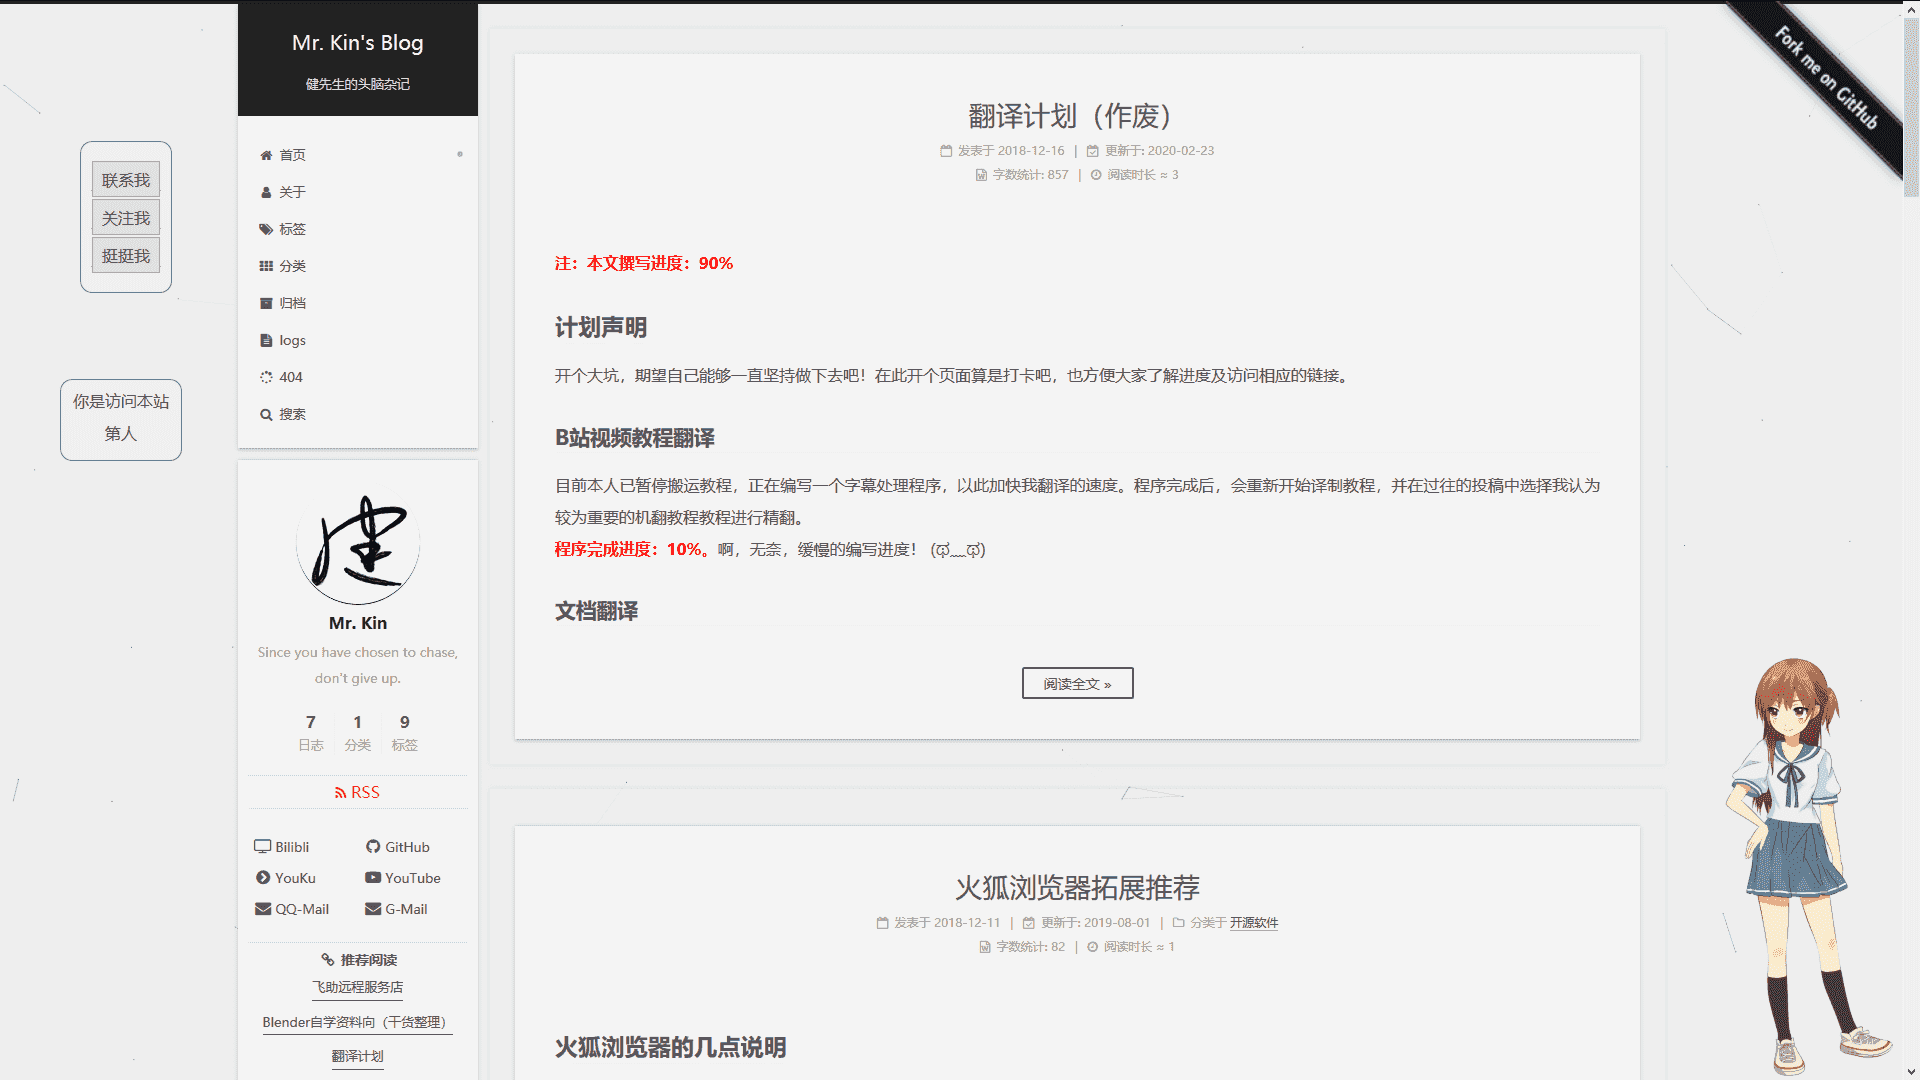
\includegraphics[scale=0.055]{Blog}
    \end{minipage}
    \qquad
    \begin{minipage}[t]{0.2\textwidth}
        \centering
        \caption*{\href{https://github.com/mister-kin}{Github}}
        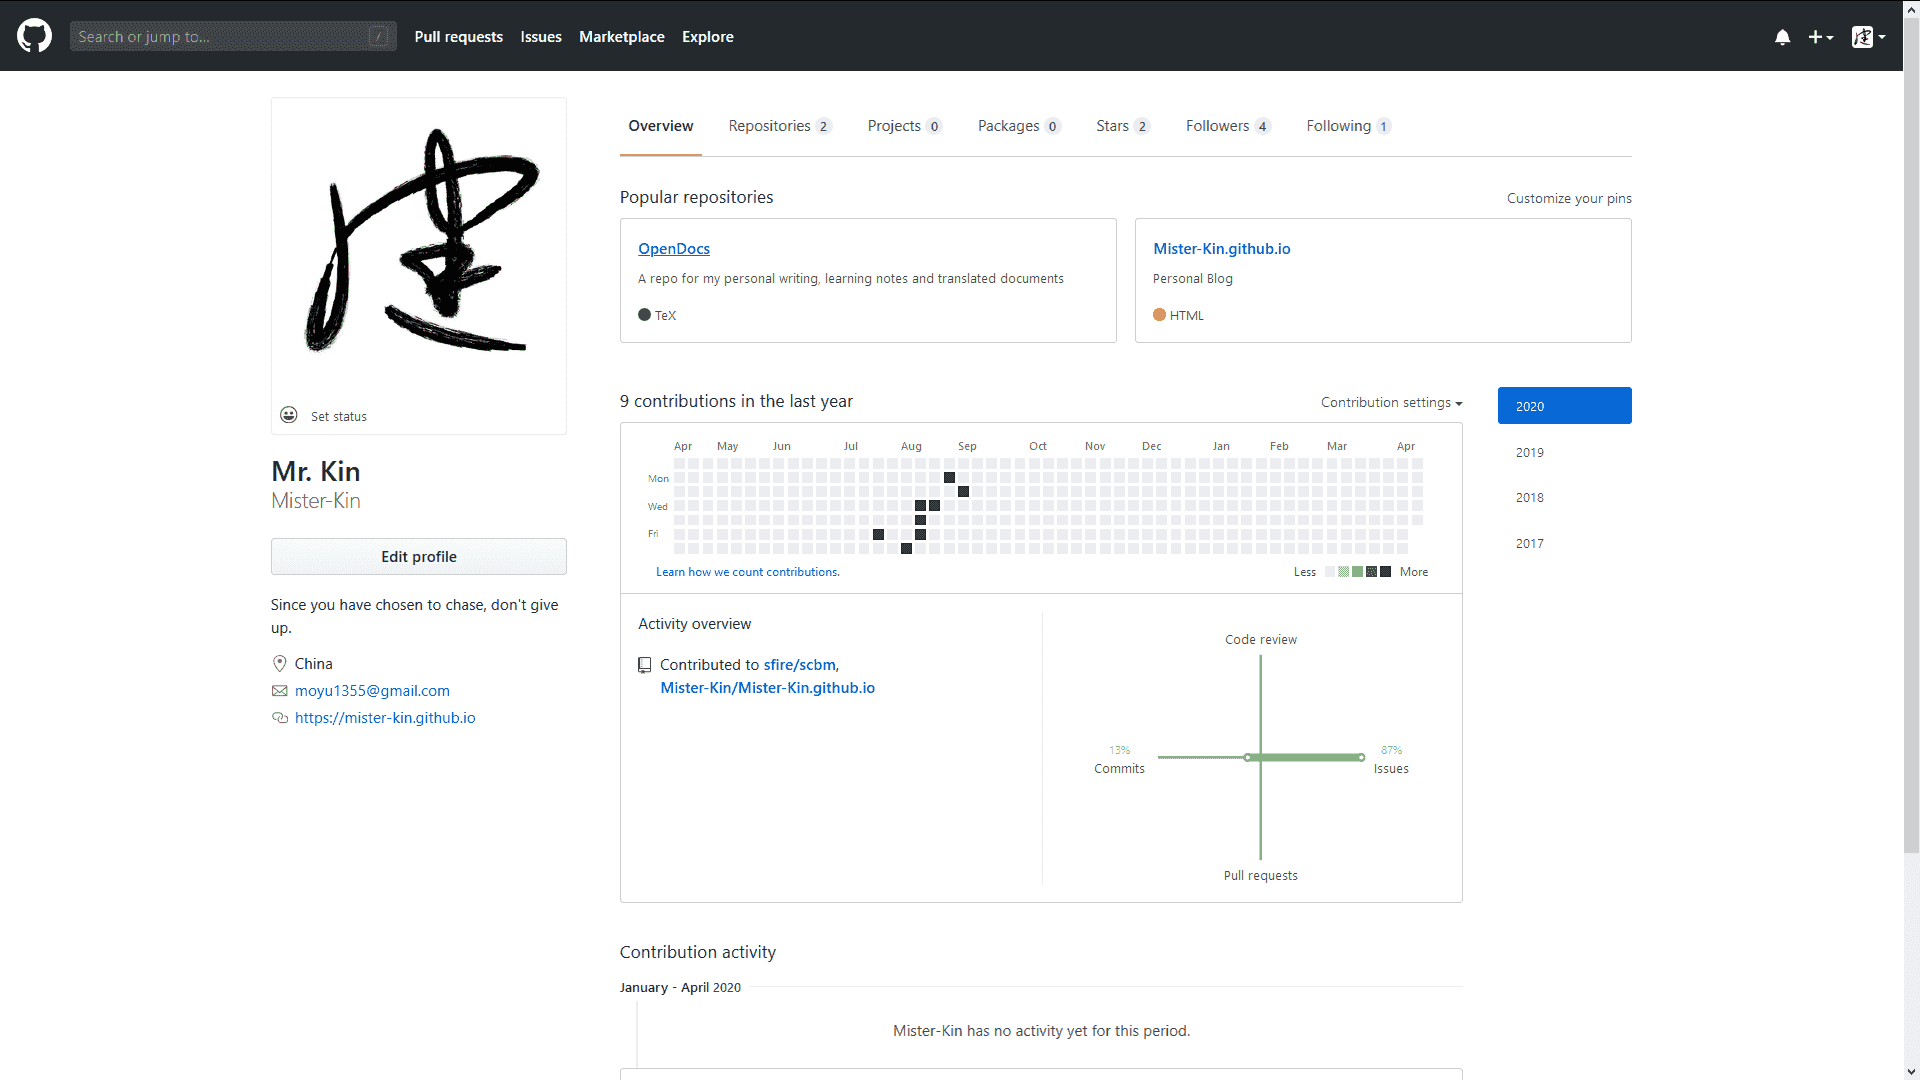
\includegraphics[scale=0.055]{Github}
    \end{minipage}
    \qquad
    \begin{minipage}[t]{0.2\textwidth}
        \centering
        \caption*{\href{https://weibo.com/6270111192/profile?topnav=1&wvr=6&is_all=1}{微博 - Weibo}}
        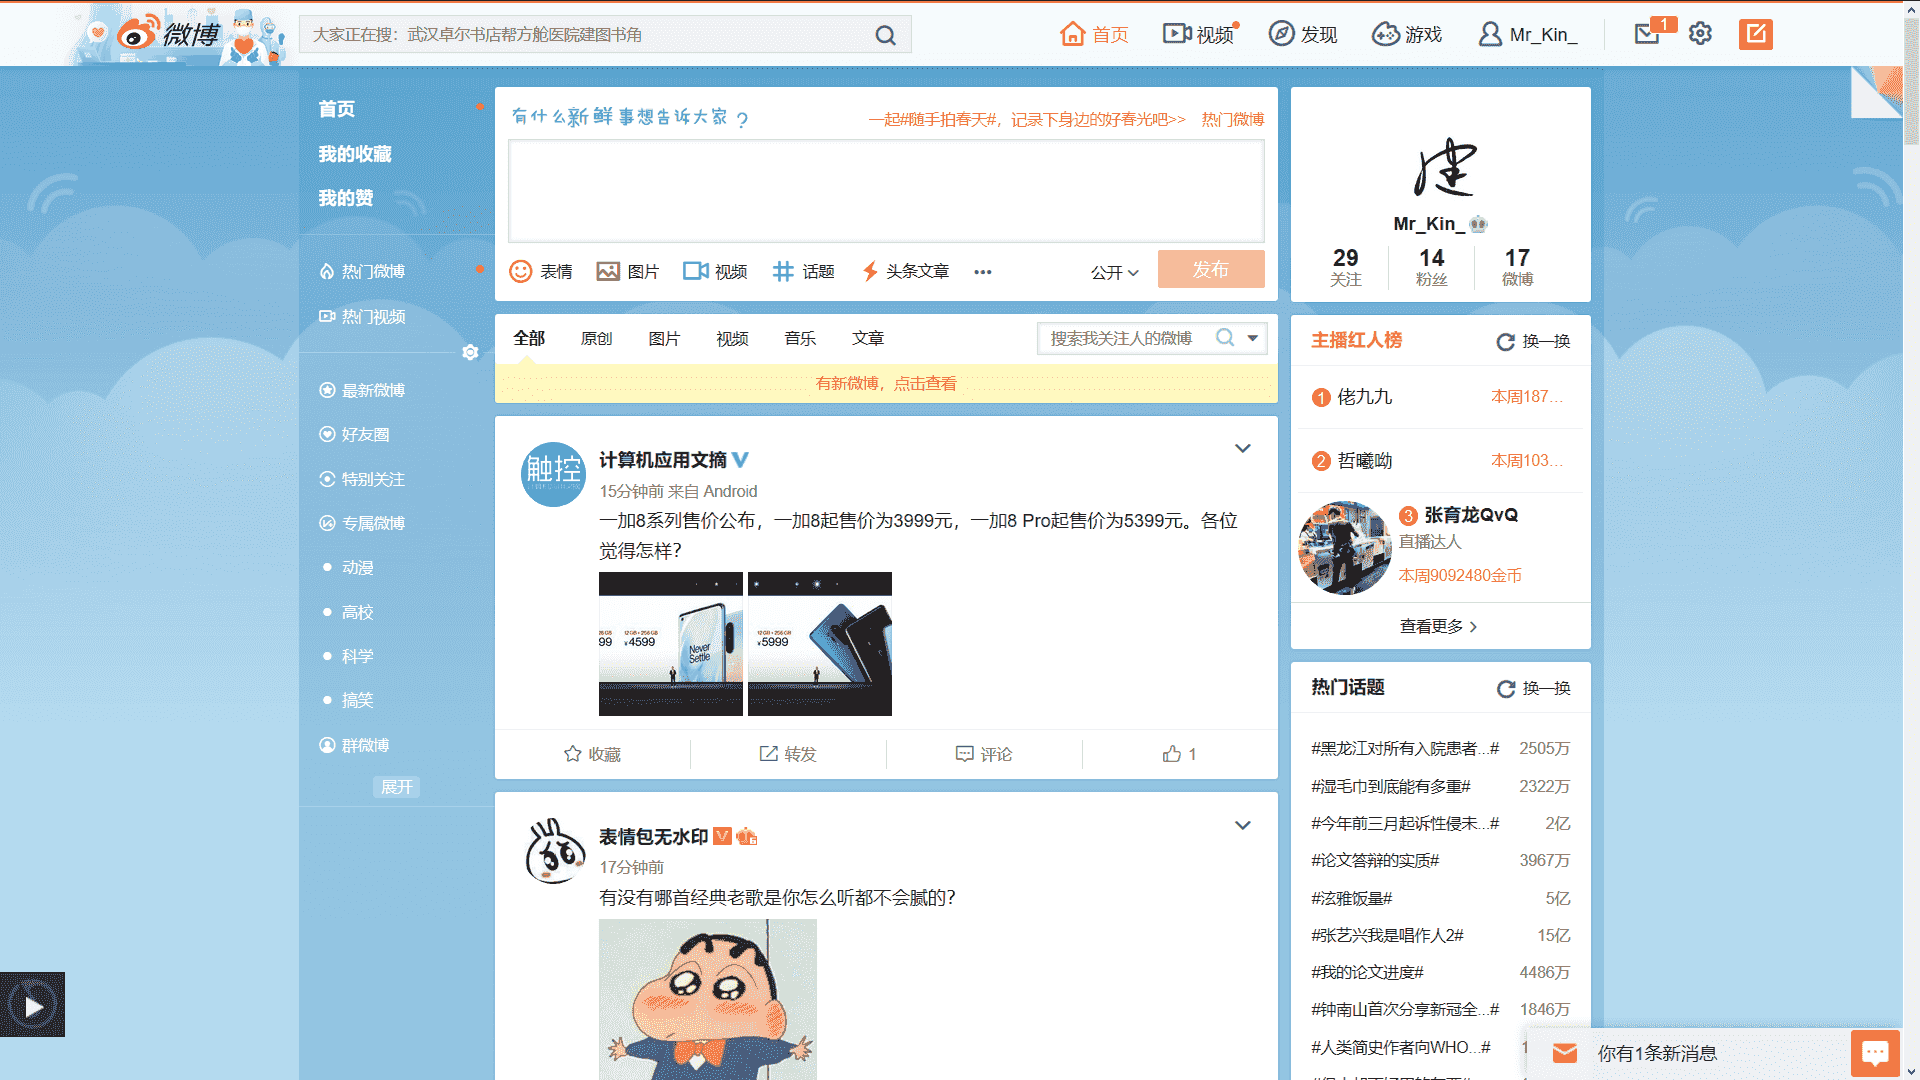
\includegraphics[scale=0.055]{Weibo}
    \end{minipage}
    \qquad
    \begin{minipage}[t]{0.2\textwidth}
        \centering
        \caption*{\href{https://www.zhihu.com/people/drwu-94}{知乎 - Zhihu}}
        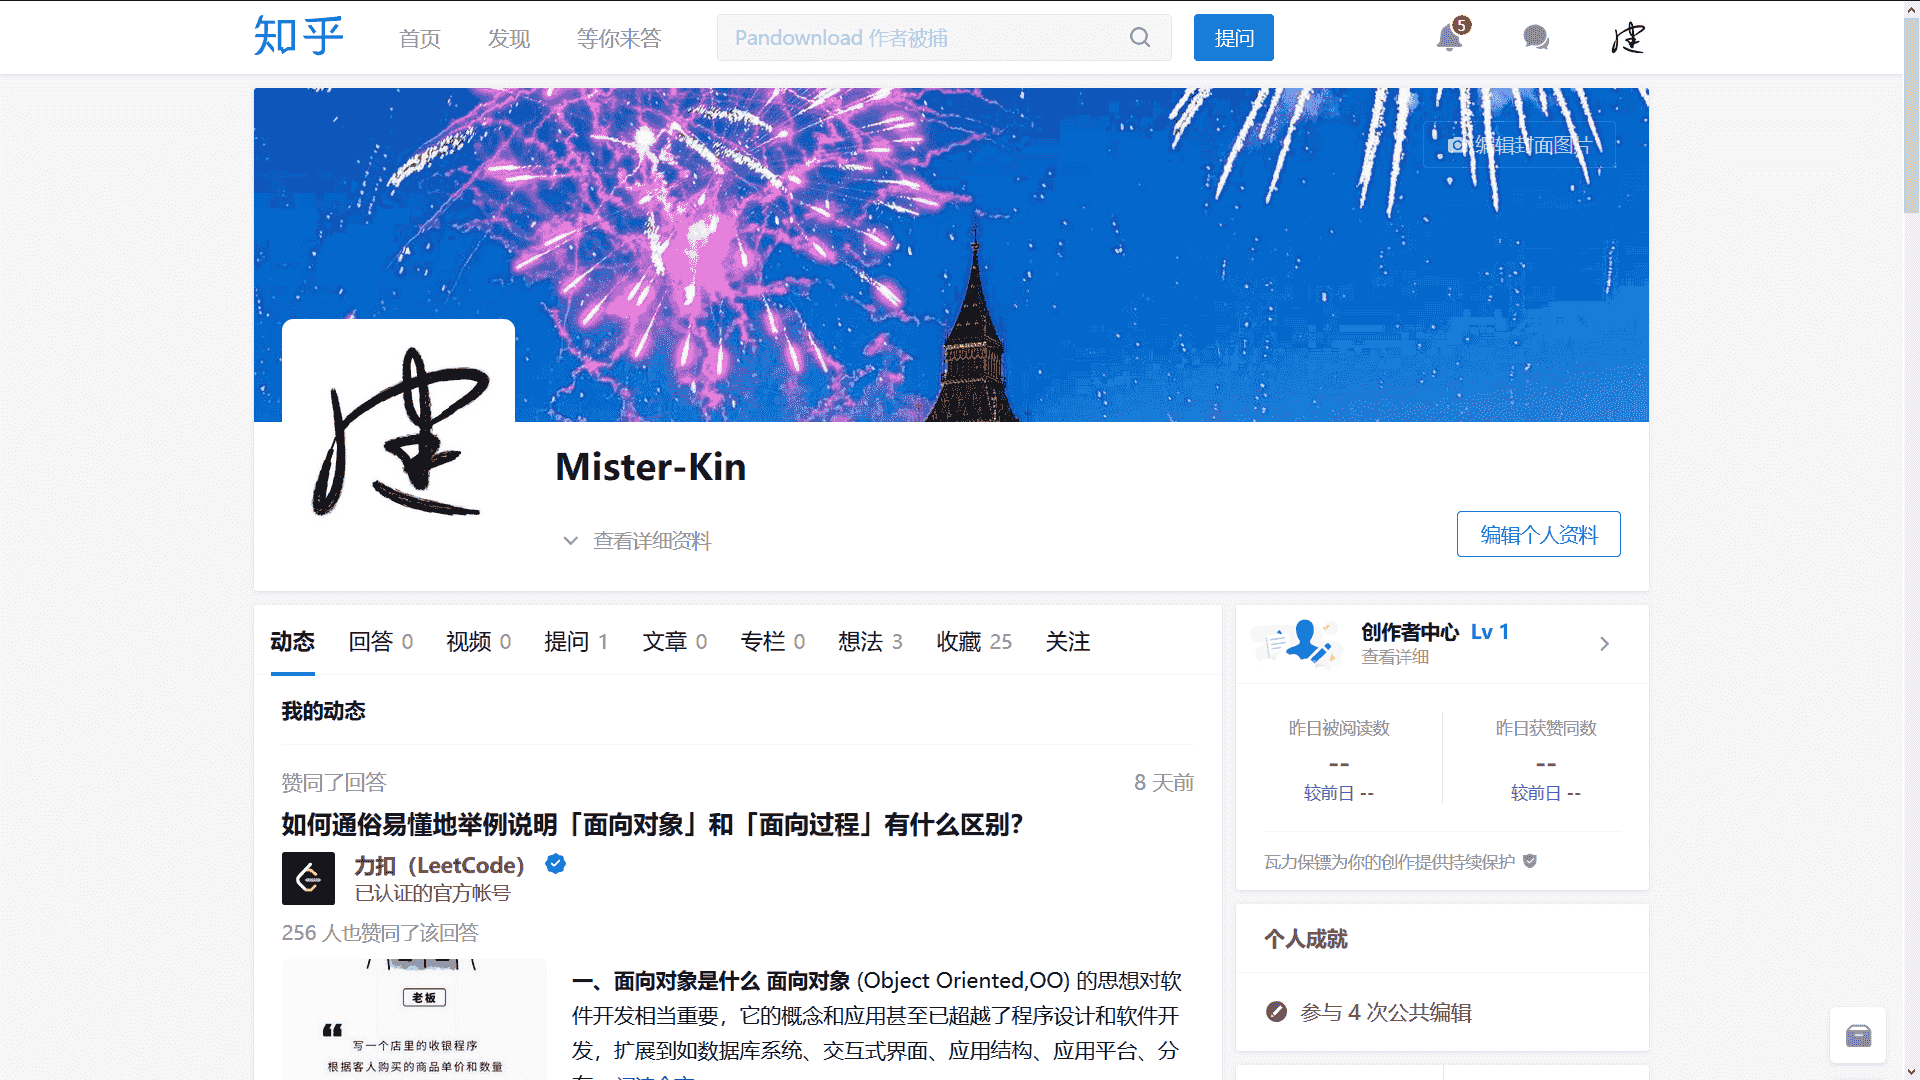
\includegraphics[scale=0.055]{Zhihu}
    \end{minipage}

    \vspace*{3ex}

    \begin{minipage}[t]{0.2\textwidth}
        \centering
        \caption*{\href{http://space.bilibili.com/17025250?}{B站 - Bilibili}}
        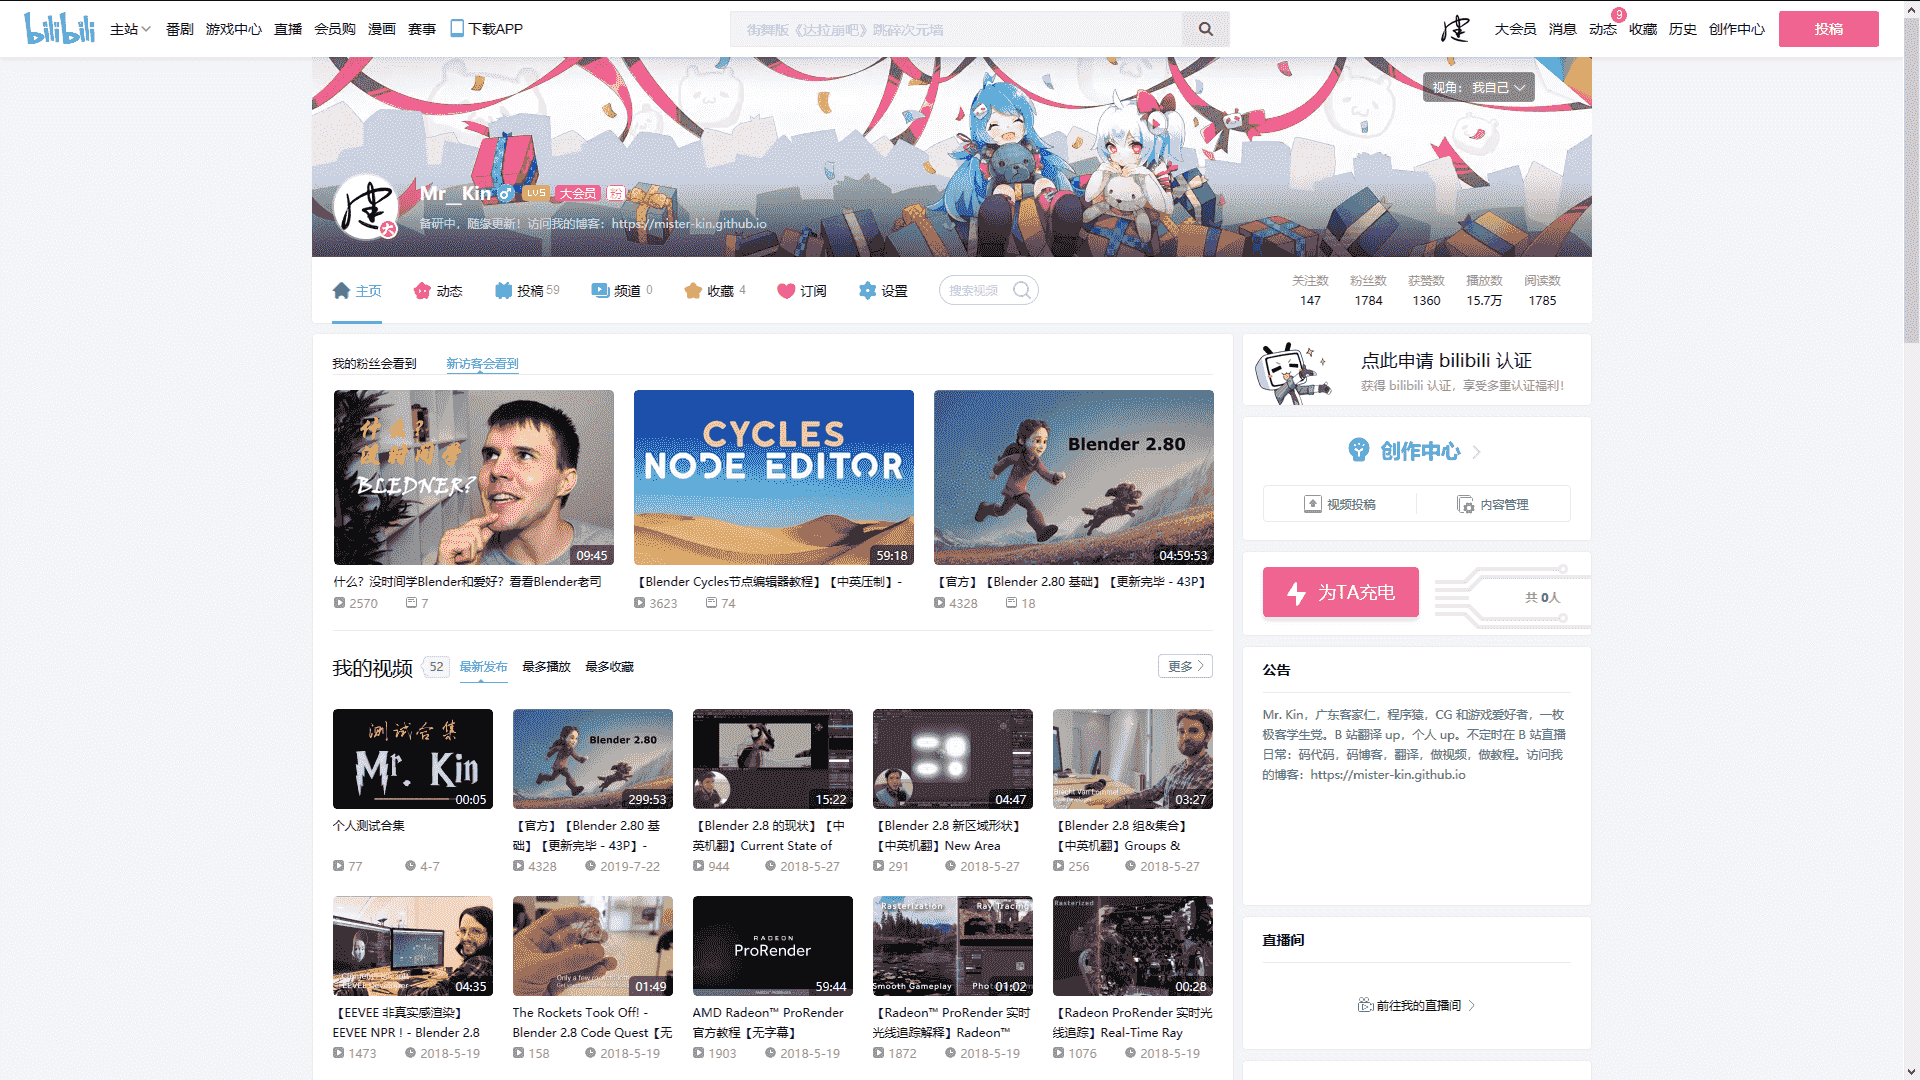
\includegraphics[scale=0.055]{Bilibili}
    \end{minipage}
    \qquad
    \begin{minipage}[t]{0.2\textwidth}
        \centering
        \caption*{\href{http://i.youku.com/i/UNjA3MTk5Mjgw?spm=a2hzp.8253869.0.0}{优酷 - Youku}}
        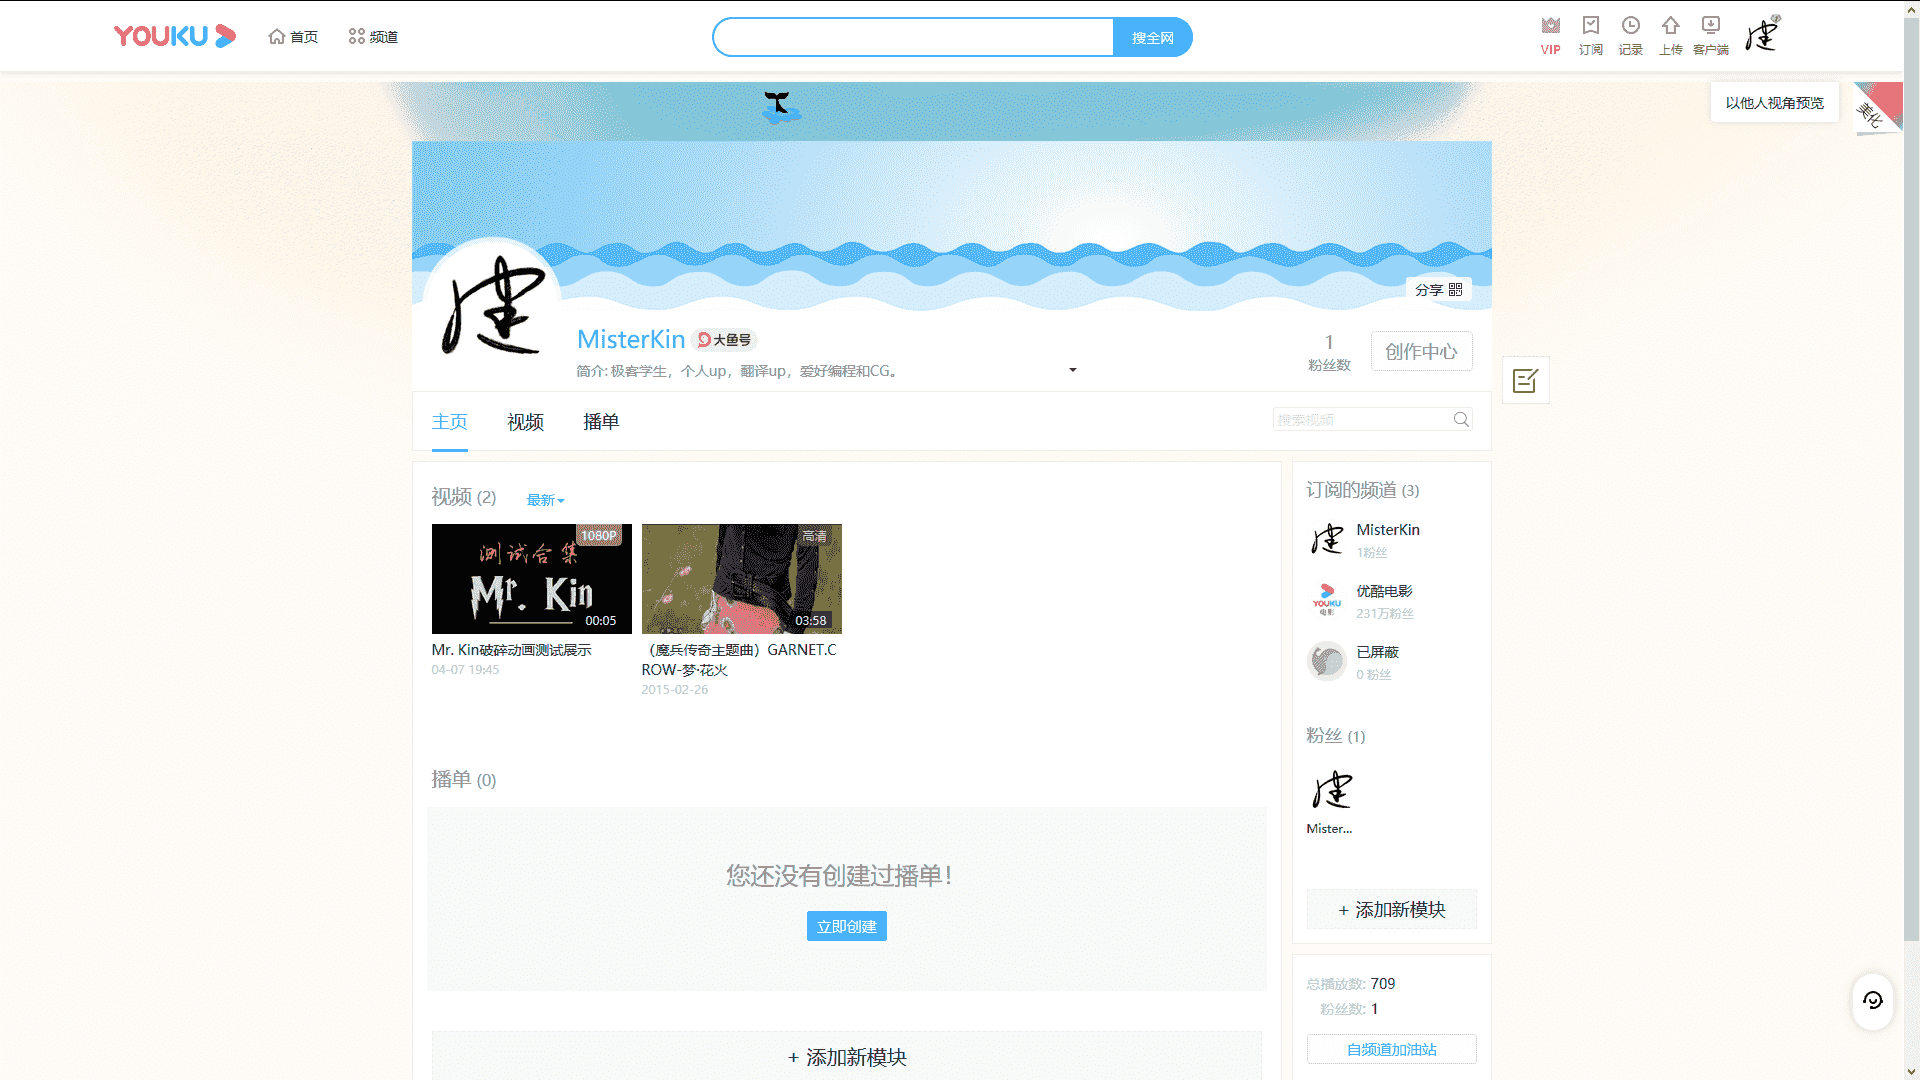
\includegraphics[scale=0.055]{Youku}
    \end{minipage}
    \qquad
    \begin{minipage}[t]{0.2\textwidth}
        \centering
        \caption*{\href{https://www.toutiao.com/c/user/835254071079053/\#mid=1663279303982091}{头条 - Headline}}
        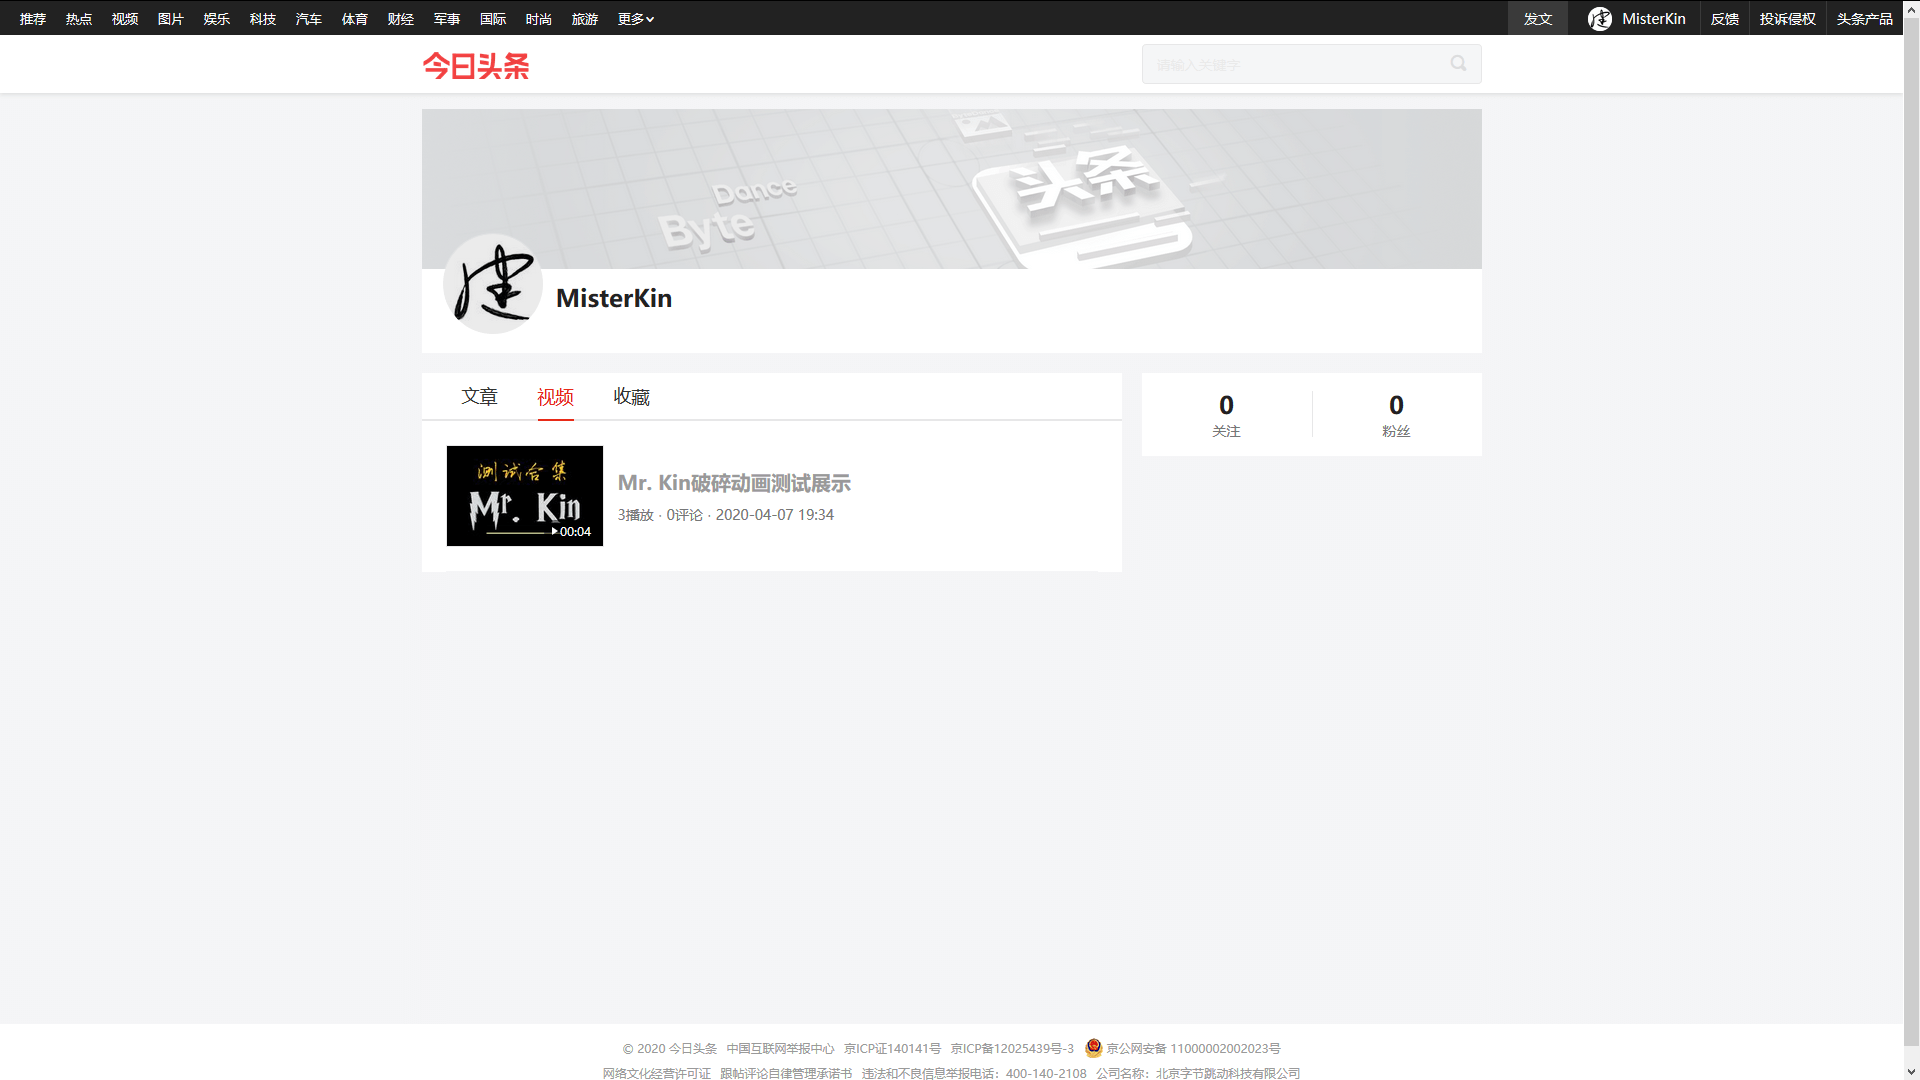
\includegraphics[scale=0.055]{Headline}
    \end{minipage}
    \qquad
    \begin{minipage}[t]{0.2\textwidth}
        \centering
        \caption*{\href{https://www.youtube.com/channel/UCXqjfWLzMlRKxGC8syWj17Q?view_as=public}{油管 - Youtube}}
        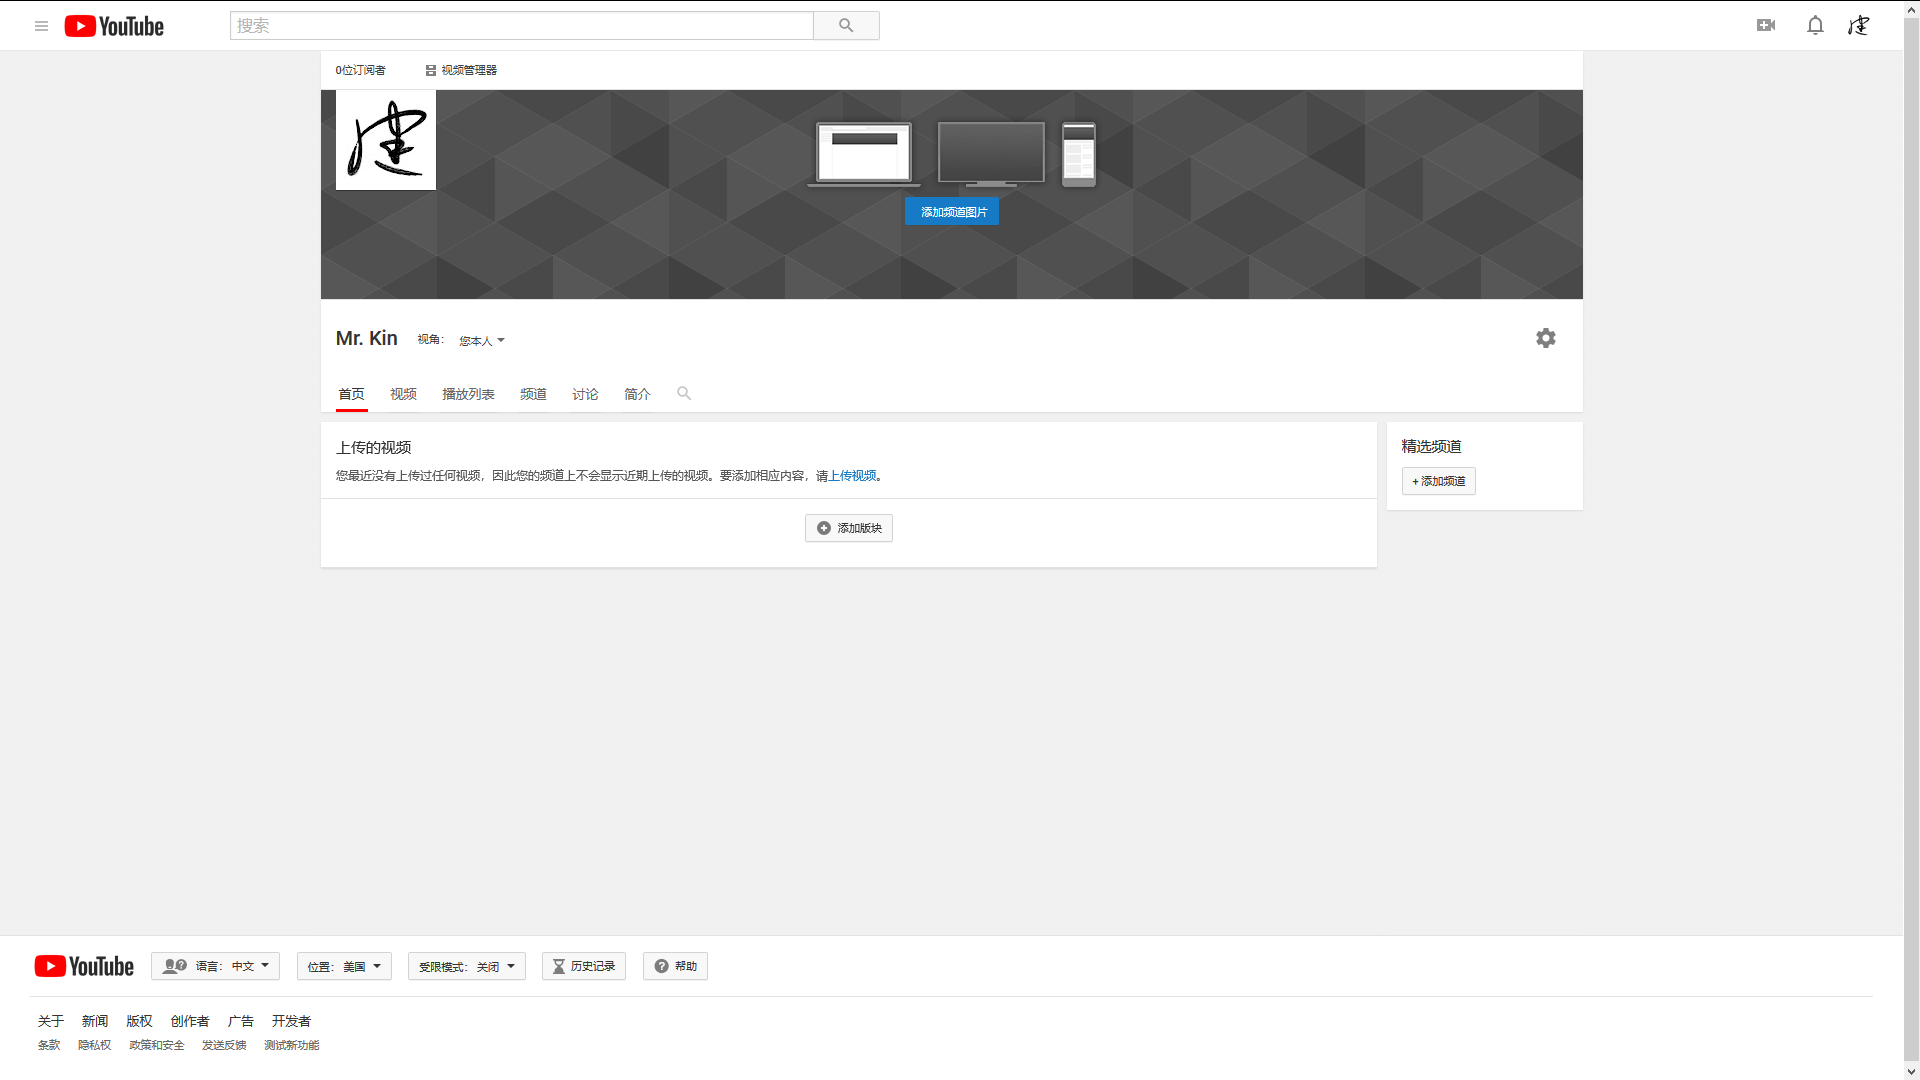
\includegraphics[scale=0.055]{Youtube}
    \end{minipage}
\end{figure}
 % 出于特殊的安全设置,\include 命令无法使用相对路径,因为需要读写权限以给 included file 写 aux 文件,而 \input 命令只需要读权限。
    \clearpage
    \phantomsection
\begin{center}
    {\bfseries\sffamily\Large 版权声明}
\end{center}
\addcontentsline{toc}{chapter}{版权声明}

\noindent 作者:Mr. Kin \\
\DetectToksEmpty\LinkBlogPost
\ifToksEmpty
博文链接:链接暂空\\
\else
博文链接:\href{\the\LinkBlogPost}{跳转博文页}\\
\fi
\DetectToksEmpty\LinkPDFSource
\ifToksEmpty
PDF及LaTex源码链接:链接暂空\\
\else
PDF及LaTex源码链接:\href{\the\LinkPDFSource}{跳转PDF及LaTex源码页}\\
\fi
\DetectToksEmpty\LinkVideo
\ifToksEmpty
\else
相关视频创作链接:\href{\the\LinkVideo}{跳转视频页}\\
\fi
许可协议:本作品的所有内容,除个人设计创作的图像(如logo等)和相关的视频创作及其他特别声明外,均采用\href{https://creativecommons.org/licenses/by-nc-sa/4.0/deed.zh}{知识共享\ 署名-非商业性使用-相同方式共享 4.0 国际许可协议}进行发布。版权 © Mr. Kin,保留所有权利。
\includegraphics[scale=.4]{CC-BY-NC-SA}\\*[1.3ex]
\begin{tabular}{|*{3}{p{0.306\textwidth}|}}
    \hline
    \textsf{\bfseries 允许} & \textsf{\bfseries 限制} & \textsf{\bfseries 条件} \\
    \hline
    \vspace{-8pt}{\color{green}√} 修改 & \vspace{-8pt}{\color{red}×} 商标使用 & \vspace{-8pt}{\color{blue}$\odot$} 保留原署名 \\[-12pt]
    {\color{green}√} 分发 & {\color{red}×} 专利使用 & {\color{blue}$\odot$} 状态变更说明 \\[-12pt]
    {\color{green}√} 个人使用 & {\color{red}×} 商业使用 & {\color{blue}$\odot$} 相同的许可和版权声明 \\
    \hline
\end{tabular}
\\*[1.3ex]
\emph{注:若想对本作品进行转载、引用亦或是进行二次创作时,请详细阅读上述相关协议内容(若不理解,请点击链接跳转阅读)。为保障本人权利,对于违反者,本人将依法予以处理!望周知!——Mr. Kin}

\begin{center}
    {\bfseries\sffamily\Large 勘误声明}
\end{center}

虽本人写作时已尽力保证其内容的正确性,但因个人知识面和经验的局限性以及计算机技术等相关技术日新月异,本作品内容或存在一些错误之处。还望诸君发现错误后能够\hyperlink{contact}{联系我}以更正错误,不胜感激!——Mr. Kin

\begin{center}
    {\bfseries\sffamily\Large 侵权声明}
\end{center}

若本作品采用的第三方内容侵犯了你的版权,请与我\hyperlink{contact}{联系}进行处理,谢谢!——Mr. Kin

\begin{center}
    {\bfseries\sffamily\Large 第三方开源许可声明}
\end{center}

\noindent 本作品使用的第三方开源产品有:
\begin{multicols}{2}
\begin{itemize}
    \item \href{https://github.com/adobe-fonts}{Adobe Fonts}: \href{https://github.com/adobe-fonts/source-serif-pro/blob/release/LICENSE.md}{OFL v1.1}
    \item \href{https://tug.org/texlive/}{Tex Live}: \href{https://tug.org/texlive/copying.html}{TeX Live Licensing}
    \item \href{https://code.visualstudio.com/}{Visual Studio Code}: \href{https://github.com/Microsoft/vscode/blob/master/LICENSE.txt}{MIT}
    \item \href{http://ffmpeg.org/}{FFmpeg}: \href{http://ffmpeg.org/legal.html}{LGPL v2.1 / GPL v2}
    \item \href{https://krita.org/en/}{Krita}: \href{https://docs.krita.org/en/KritaFAQ.html?highlight=license#license-rights-and-the-krita-foundation}{Krita's GPL license}
    \item \href{https://inkscape.org/}{Inkscape}: \href{https://inkscape.org/about/license/}{GPL}
    \item \href{https://www.gimp.org}{GIMP}: \href{https://www.gimp.org/about/COPYING}{GPL}
    \item \href{https://www.blender.org}{Blender}: \href{https://www.blender.org/about/license/}{GPL}
    \item \href{https://www.audacityteam.org/}{Audacity}: \href{https://www.audacityteam.org/about/license/}{GPL v2}
    \item \href{https://handbrake.fr}{Handbrake}: \href{https://github.com/HandBrake/HandBrake/blob/master/LICENSE}{GPL v2}
\end{itemize}
\end{multicols}

\noindent 更多请点击查看\href{https://mister-kin.github.io/about/third-party-declaration/}{第三方声明页}!

    \clearpage
    {\centering \tableofcontents} % 生成目录页。
    \mainmatter

    % 正文
    \part{中文字体测试}
    \chapter{章标题测试}
    \section{节标题测试}
    \subsection{子节标题测试}
    \subsubsection{子子标题测试}
    \paragraph{段标题测试}
    测试
    \subparagraph{子段标题测试}
    测试

    \subsection{字体样式测试}
    {\rmfamily 思宋:测试 \textbf{粗体:测试} \textup{直立体:测试} \textit{意大利斜体:测试} \textsl{倾斜体:测试}}

    {\sffamily 思黑:测试 \textbf{粗体:测试} \textup{直立体:测试} \textit{意大利斜体:测试} \textsl{倾斜体:测试}}

    \subsection{字体测试}
    {\rmfamily 思宋:滚滚长江东逝水,浪花淘尽英雄。是非成败转头空,青山依旧在,几度夕阳红。白发渔樵江渚上,惯看秋月春风。一壶浊酒喜相逢,古今多少事,都付笑谈中。}

    {\sffamily 思黑:滚滚长江东逝水,浪花淘尽英雄。是非成败转头空,青山依旧在,几度夕阳红。白发渔樵江渚上,惯看秋月春风。一壶浊酒喜相逢,古今多少事,都付笑谈中。}

    \part{English Font Test}
    \chapter{Chapter Title Test}
    \section{Section Title Test}
    \subsection{Subsection Title Test}
    \subsubsection{Subsubsection Title Test}
    \paragraph{Paragraph Title Test}
    Test
    \subparagraph{Subparagraph Title Test}
    Test

    \subsection{Font Format Test}
    {\rmfamily textrm: test \textbf{textbf:test} \textup{textup:test} \textit{textit:test} \textsl{textsl:test}}

    {\sffamily textsf: test \textbf{textbf:test} \textup{textup:test} \textit{textit:test} \textsl{textsl:test}}

    {\ttfamily texttt: test \textbf{textbf:test} \textup{textup:test} \textit{textit:test} \textsl{textsl:test}}

    \subsection{Font Test}
    {\rmfamily textrm: The quick brown fox jumps over the lazy dog}

    {\sffamily textsf: The quick brown fox jumps over the lazy dog}

    {\ttfamily texttt: The quick brown fox jumps over the lazy dog}

    \subsection{IPA Test}
    anode \ipa{'ænoʊd}

    cathode \ipa{'kæθoʊd}

    \chapter{各类测试}

    \begin{intro}
        intro环境测试。intro 环境,用以章节开头的文字介绍。排版上比普通正文多缩进两个文字。
    \end{intro}

    \paragraph{普通文字段} 滚滚长江东逝水,浪花淘尽英雄。是非成败转头空,青山依旧在,几度夕阳红。白发渔樵江渚上,惯看秋月春风。一壶浊酒喜相逢,古今多少事,都付笑谈中。

    \paragraph{有序列表}
    \begin{enumerate}[label={Step \arabic*.}]
        \item test
        \item test
        \item test
        \item 滚滚长江东逝水,浪花淘尽英雄。是非成败转头空,青山依旧在,几度夕阳红。白发渔樵江渚上,惯看秋月春风。一壶浊酒喜相逢,古今多少事,都付笑谈中。
    \end{enumerate}

    \paragraph{无序列表}
    \begin{itemize}
        \item test
        \item test
        \item test
        \item 滚滚长江东逝水,浪花淘尽英雄。是非成败转头空,青山依旧在,几度夕阳红。白发渔樵江渚上,惯看秋月春风。一壶浊酒喜相逢,古今多少事,都付笑谈中。
    \end{itemize}

    \begin{lstlisting}[language={C},title={\textsf{C语言代码段测试}}]
        for(,1,);
        printf("Hello World!"); // 注释测试 Test
    \end{lstlisting}

    \paragraph{\color{black}颜色测试}
    {\color{red} 红色}

    \paragraph{下划线测试}
    \uline{下划线}
    \uuline{双下划线}
    \uwave{波浪线}
    \sout{删除线}
    \xout{斜线}
    \dashuline{下划线-虚线}
    \dotuline{下划线-点}

    \rmnum{3}

    \Rmnum{3} $K_{test}^{\text{\Rmnum{3}}}$ $K_{test}^{\mathrm{\Rmnum{3}}}$ $\Delta Q$

    \newpage
    \noindent {\bfseries \sffamily 图片测试}
    \begin{figure}[h!]
        \centering
        
\includegraphics[scale=0.9]{SampleImage}
        \caption{示例图片}
    \end{figure}

    \nocite{*} % 不使用 cite 也能生成参考文献。
    \printbibliography % 生成参考文献排版。
    \addcontentsline{toc}{chapter}{参考文献} % 添加参考文献进目录。

    \appendix
    % 附录
    \chapter{附录测试1}
    \section{节测试}
    \subsection{子节测试}
    \chapter{附录测试2}

\end{document}
